\documentclass[CJKutf8,xcolor=pdftex,dvipsnames,table]{beamer}
\usepackage{hyperref}
\hypersetup{
  pdftitle={Operating System Concepts},
  pdfauthor={Hong MingJian},
  pdfsubject={Memory Management},
  pdfpagemode={FullScreen},
  colorlinks={true},
  linkcolor={blue},
}
\usepackage{CJKutf8}

\usetheme{Madrid}%{Warsaw}
\usecolortheme{crane}

%gets rid of bottom navigation bars
\setbeamertemplate{footline}[page number]{}
%gets rid of navigation symbols
\setbeamertemplate{navigation symbols}{}

\begin{document}
\begin{CJK*}{UTF8}{song}

  \title{\CJKfamily{hei} 操作系统原理}
  \subtitle{\CJKfamily{hei} 第九章:内存管理}
	\author{\CJKfamily{hei} 洪明坚}
	\institute{\CJKfamily{hei} 重庆大学软件学院}
  \date{\today}

  \AtBeginSection[]
  {
    \begin{frame}
      \frametitle{Outline}
      \tableofcontents[currentsection]
    \end{frame}
  }

  \frame{\titlepage}
  \frame{\frametitle{目录}\tableofcontents}

  \section{内存管理介绍}
  
  %% PAGE
  \begin{frame}
    \frametitle{内存管理介绍} \pause
    \begin{itemize}
    \item{进程管理回顾} \pause
      \begin{itemize}
      \item{进程管理提供了一个虚拟的机器接口,让每一个进程都以为是自己在独占CPU,如下图所示:} \pause
        \begin{center}
          \includegraphics[scale=.4]{pm} \pause
        \end{center}
      \end{itemize}
    \item{内存管理的任务} \pause
      \begin{itemize}
      \item{提供一个虚拟的机器接口,让每一个进程都以为是自己在独占RAM。}
      \end{itemize}
    \end{itemize}
  \end{frame}
  
  %% PAGE
  \begin{frame}
  \frametitle{Questions}
  \begin{itemize}
  \item{Any questions?}
  \end{itemize}
  \begin{center}
    
\includegraphics[scale=.5]{question}
  \end{center}
  \end{frame}

  \section{基本方法}

  %% PAGE
  \begin{frame}
  \frametitle{基本方法 - 以MS-DOS为例} \pause
  \begin{minipage}[c]{0.6\textwidth}
    \begin{itemize}
    \item{MS-DOS (Microsoft Disk Operating System)} \pause
      \begin{itemize}
      \item{单用户、单任务} \pause
      \item{只能访问1MB内存} \pause
        \begin{itemize}
        \item{INTEL 8086/80286只有20根地址线} \pause
        \end{itemize}
      \item{没有任何保护机制} \pause
        \begin{itemize}
        \item{INTEL 8086/80286没有提供硬件保护机制支持} \pause
        \end{itemize}
      \end{itemize}
    \end{itemize}
  \end{minipage}%
  \begin{minipage}[c]{0.4\textwidth}
    \centering
    \includegraphics[scale=0.5]{msdos} \\ \pause
    640K should be enough for anybody -- Bill Gates
  \end{minipage}
  \end{frame}

  %% PAGE
  \begin{frame}
  \frametitle{问题(一)} \pause
  \begin{itemize}
  \item{在MS-DOS中,}  \pause
    \begin{itemize}
    \item{MS-DOS自己要占用1/3左右;} \pause
    \item{剩余部分留给系统\textbf{唯一}的进程使用。} \pause
    \end{itemize}
  \item{问题}  \pause
    \begin{itemize}
    \item{如果某个MS-DOS下的应用程序需要超过640K的内存才能运行,怎么办?} \pause
    \end{itemize}
  \item{Solution} \pause
    \begin{itemize}
    \item{\textbf{Overlay}: A technique to enable a process to be larger than the amount of memory allocated to it.} \pause
    \item{The idea of overlay is keeping in memory only those instructions and data that are needed at any given time.}
    \end{itemize}
  \end{itemize}
  \end{frame}
  
  %% PAGE
  \begin{frame}
  \frametitle{Overlay: An example}
  \begin{itemize}
  \item{A two-pass assembler \pause}
    \begin{itemize}
    \item{Pass 1: 扫描源代码,找到所有的符号并构造符号表(symbol table);} \pause
    \item{Pass 2: 根据前面的符号表产生机器代码。} \pause
    \end{itemize}
  \item{为一致起见,假设} \pause
    \begin{itemize}
    \item{系统目前只有150K内存可以使用,而该assembler需要200K的内存才能运行;} \pause
    \item{该assembler在运行时主要包括如下模块,} \pause
      \begin{itemize}
      \item{Pass 1,需要70K内存;} \pause
      \item{Pass 2,需要80K内存;} \pause
      \item{符号表,需要20K内存;} \pause
      \item{Pass 1和2共用代码(common routines),需要30K内存。}
      \end{itemize}
    \end{itemize}
  \end{itemize}
  \end{frame}
  
  %% PAGE
  \begin{frame}
  \frametitle{Overlay: How to do?} \pause
  \begin{itemize}
  \item{程序员根据程序的特点,将一些独立的模块根据需要调入内存,覆盖已经使用过的模块,如下图所示:} \pause
  \item{除了程序本身外,程序员还要提供一个所谓的“overlay driver”来负责模块的调入调出。} \pause
  \end{itemize}
  \begin{center}
    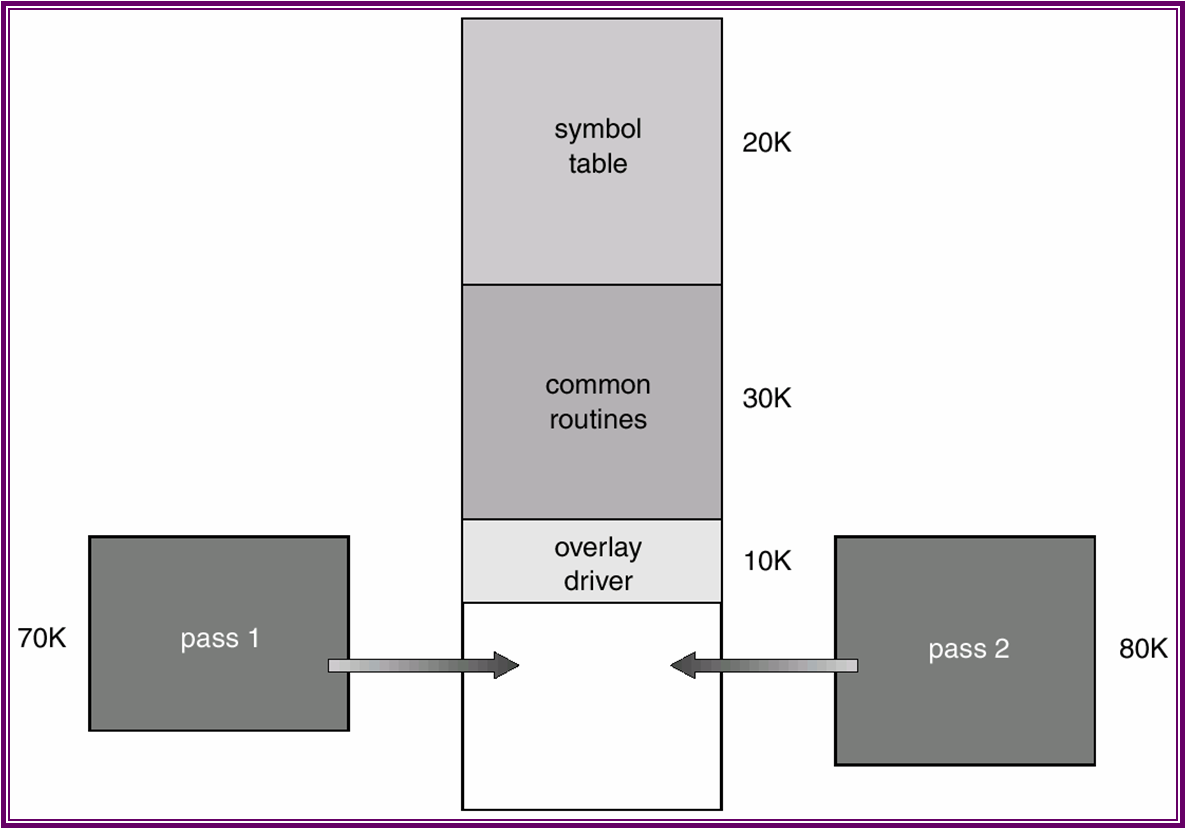
\includegraphics[scale=0.4]{v6f9-3}
  \end{center}
  \end{frame}
  
  %% PAGE
  \begin{frame}
  \frametitle{Overlay: 结论} \pause
  \begin{itemize}
  \item{前面的例子是最简单情况下的overlay。一般情况下,对复杂的系统进行overlay要求开发人员对系统进行精心的设计和实现,需要很高的技巧;} \pause
  \item{因此,目前这种技术已经很少被使用,除了在一些内存资源相当紧张的嵌入式系统中;} \pause
  \item{但是,Overlay的思想非常重要:} \pause
    \begin{itemize}
    \item{无论进程在运行时占有多大的内存,在某一段时间内,它只会访问其中的一部分。}
    \end{itemize}
  \end{itemize}
  \end{frame}
  
  %% PAGE
  \begin{frame}
  \frametitle{Questions}
  \begin{itemize}
  \item{Any questions?}
  \end{itemize}
  \begin{center}
    
\includegraphics[scale=.5]{question}
  \end{center}
  \end{frame}

  %% PAGE
  \begin{frame}
  \frametitle{问题(二)} \pause
  \begin{itemize}
  \item{假设MS-DOS支持多任务,即系统中有多个进程。当然,}  \pause
    \begin{itemize}
    \item{进程必须在内存中才能运行;}  \pause
    \item{运行中的进程可能会申请额外的内存。}  \pause
    \end{itemize}
  \item{问题} \pause
    \begin{itemize}
    \item{假设系统目前有两个进程:$P_1$和$P_2$,而且系统已经没有内存可以使用。此时,正在运行的$P_1$又要申请更多的内存才能继续运行,怎么办?} \pause
    \end{itemize}
  \item{Solution} \pause
    \begin{itemize}
    \item{\textbf{Swap}: A process can be swapped temporarily out of memory to a backing-store, and then brought into memory for continued execution.}
    \end{itemize}
  \end{itemize}
  \end{frame}
  
  %% PAGE
  \begin{frame}
  \frametitle{Swap: How to do?} \pause
  \begin{itemize}
  \item{此时,OS可以将(不在运行的)$P_2$交换到backing-store中;同时释放$P_2$所占用的内存,并分配给$P_1$让其继续运行。} \pause
  \item{当调度器重新调度$P_2$运行时,OS从backing-store中加载$P_2$到内存继续运行。} \pause
    \begin{itemize}
    \item{此时可能要把$P_1$交换到backing-store中以释放足够的内存空间供$P_2$运行。} \pause
    \end{itemize}
  \end{itemize}
  \begin{center}
    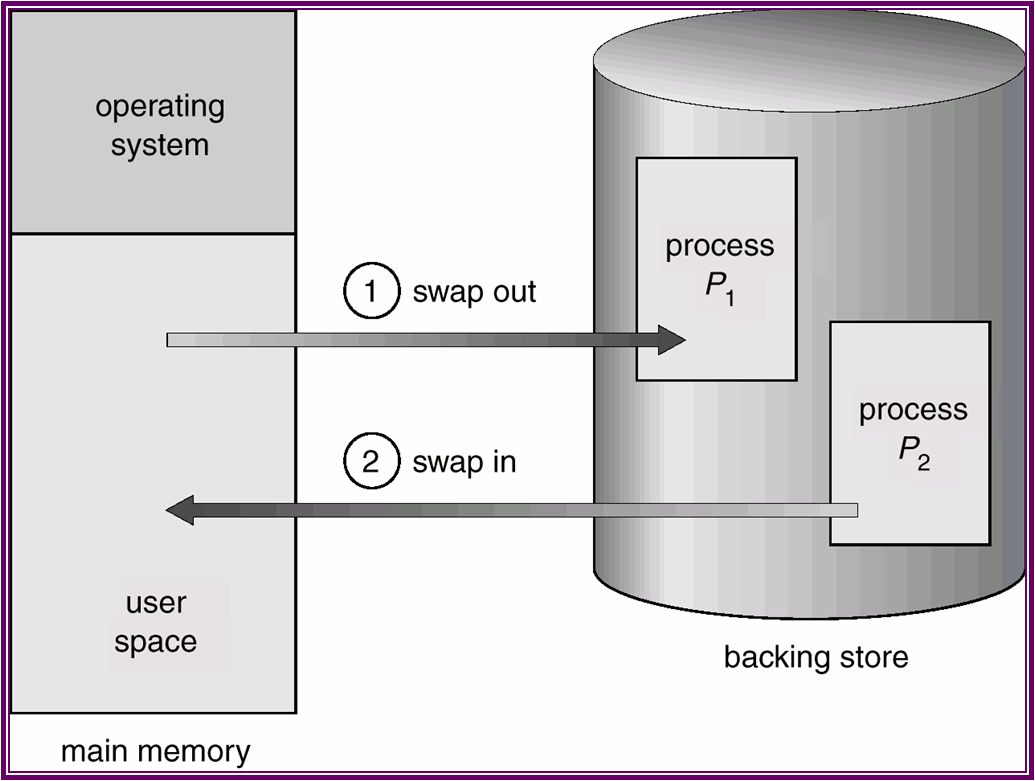
\includegraphics[scale=.3]{v6f9-4}
  \end{center}
  \end{frame}
  
  %% PAGE
  \begin{frame}
  \frametitle{Swap: 结论} \pause
  \begin{itemize}
  \item{Swap方法存在的限制:} \pause
    \begin{itemize}
    \item{要求计算机必须配备足够大的backing-store;} \pause
      \begin{itemize}
      \item{backing-store一般是快速、大容量的硬盘。} \pause
      \end{itemize}
    \item{Context switch要花费大量的时间:} \pause
      \begin{itemize}
      \item{主要用于磁盘数据传输。因此,} \pause
      \item{调度算法的设计尤其重要,应尽量减少context switch。} \pause
      \end{itemize}
    \item{被swap-out的进程必须被重新swap-in到相同的内存地址才能继续运行。} \pause
    \end{itemize}
  \item{因此,这种原始的swap-in/out已经很少被使用。} \pause
  \item{但是,swap的思想非常重要:} \pause
    \begin{itemize}
    \item{当系统内存不足时,可以向backing-store“借”一部分来使用。}
    \end{itemize}
  \end{itemize}
  \end{frame}
  
  %% PAGE
  \begin{frame}
  \frametitle{Questions}
  \begin{itemize}
  \item{Any questions?}
  \end{itemize}
  \begin{center}
    
\includegraphics[scale=.5]{question}
  \end{center}
  \end{frame}
  
  %% PAGE
  \begin{frame}
  \frametitle{多任务系统的内存管理} \pause
  \begin{itemize}
  \item{多任务环境下会带来许多内存管理问题:} \pause
    \begin{itemize}
    \item{重定位(relocation)问题;} \pause
    \item{内存保护(protection)问题;} \pause
    \item{内存分配(allocation)问题。} \pause
    \end{itemize}
  \item{下面将逐一展开讲解。}
  \end{itemize}
  \end{frame}

  %% PAGE
  \begin{frame}
  \frametitle{Relocation: 背景} \pause
  \begin{minipage}[c]{0.6\textwidth}
    \begin{itemize}
    \item{源程序变成进程的过程:} \pause
      \begin{itemize}
      \item{程序员编写的代码(source code)必须先被编译成目标文件(object file);} \pause
      \item{然后通过链接器(linkage editor)链接成可执行文件(executable);} \pause
      \item{最后由操作系统加载可执行文件到内存从而形成进程,如图所示。} \pause
      \end{itemize}
    \end{itemize}
  \end{minipage}%
  \begin{minipage}[c]{0.4\textwidth}
    \centering
    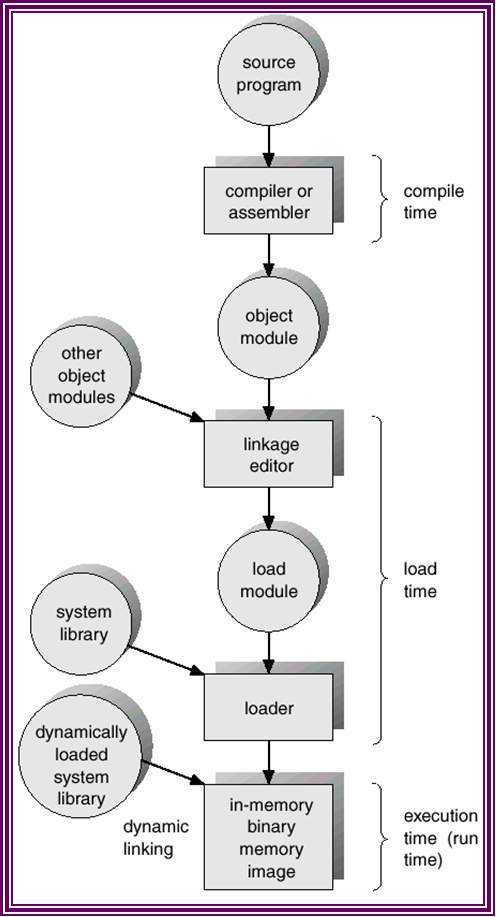
\includegraphics[scale=0.5]{v6f9-1}
  \end{minipage}
  \end{frame}
  
  %% PAGE
  \begin{frame}
  \frametitle{Relocation: 概念} \pause
  \begin{itemize}
  \item{在多任务的环境中,可执行文件可能会被加载到内存中的任何位置运行。} \pause
  \item{链接器在生成可执行文件时必须确定程序中各个符号(如函数、全局变量)的地址。} \pause
    \begin{itemize}
    \item{把程序中的符号映射为地址的过程叫做地址绑定(address binding)。} \pause
    \end{itemize}
  \item{事实上,由于链接器无法预知程序将被加载到哪个内存位置,因此无法完成\textbf{绝对的}地址绑定。} \pause
    \begin{itemize}
    \item{因此,链接器只能假定程序中第一条指令的地址是0,从而用相对于它的偏移量来进行\textbf{相对的}地址绑定;} \pause
    \item{这样的程序只能被加载到0地址的内存运行;如果该程序被加载到其他非0的地址,必须对程序中所引用的地址进行修改才能运行,这个修改过程就称为重定位。}
    \end{itemize}
  \end{itemize}
  \end{frame}
  
  %% PAGE
  \begin{frame}
  \frametitle{Relocation: How to do?} \pause
  \begin{itemize}
  \item{几个概念:} \pause
    \begin{itemize}
    \item{逻辑地址(logical address)指程序中引用的地址,亦即CPU产生的地址;} \pause
    \item{物理地址(physical address)指系统中内存单元所看到的地址;} \pause
    \item{内存管理单元(Memory Management Unit, MMU)指专门完成逻辑地址到物理地址转换的硬件单元,一般是CPU的一部分。} \pause
    \end{itemize}
    \begin{minipage}[c]{0.4\textwidth}
    \item{假设某个程序被加载到地址14000运行,正在访问逻辑地址为346的内存,如图所示:} \pause
    \end{minipage}%
    \begin{minipage}[c]{0.6\textwidth}
      \centering
      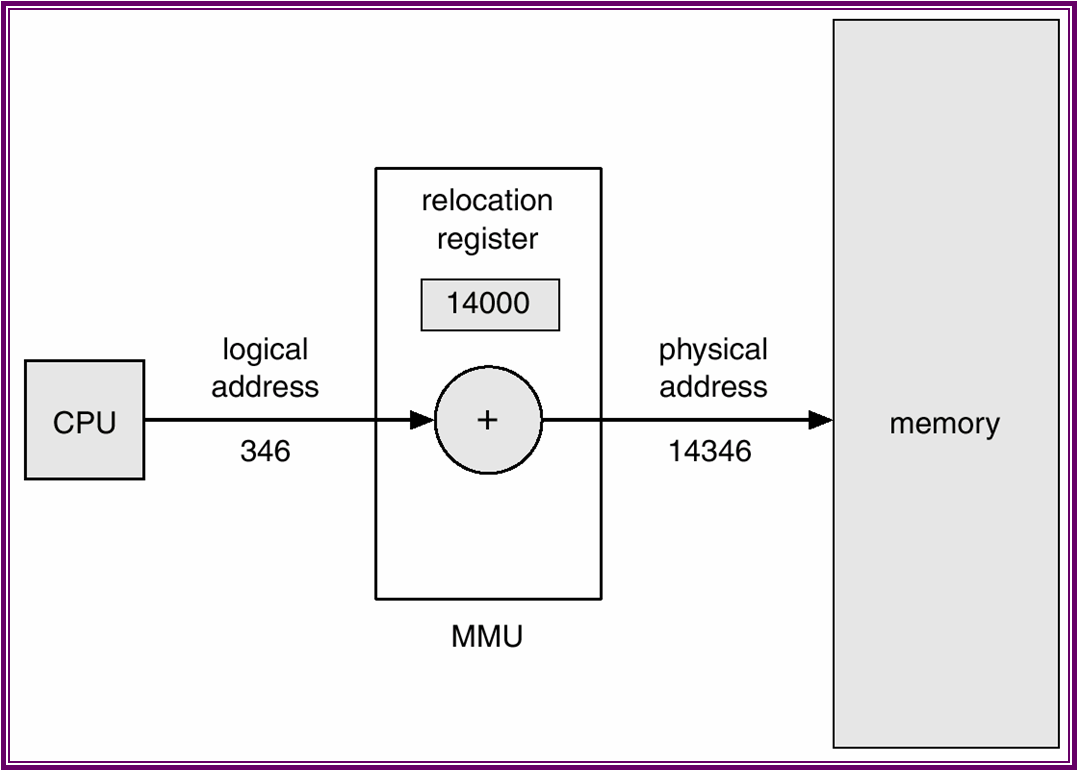
\includegraphics[scale=.3]{v6f9-2}
    \end{minipage}
  \end{itemize}
  \end{frame}
  
  %% PAGE
  \begin{frame}
  \frametitle{Relocation: 结论} \pause
  \begin{itemize}
  \item{前面介绍的是最简单的重定位技术,只是冰山的一角;} \pause
  \item{我们今天使用的操作系统(如Windows,Linux)所采用的重定位技术相当复杂,涉及到编译器、链接器、可执行文件、函数库、操作系统内核和硬件等多个组件之间的协作才能完成;} \pause
  \item{在讲完虚拟内存技术后,我们将继续深入讲解这部分内容。}
  \end{itemize}
  \end{frame}
  
  %% PAGE
  \begin{frame}
  \frametitle{Questions}
  \begin{itemize}
  \item{Any questions?}
  \end{itemize}
  \begin{center}
    
\includegraphics[scale=.5]{question}
  \end{center}
  \end{frame}

  %% PAGE
  \begin{frame}
  \frametitle{Protection: 问题} \pause
  \begin{itemize}
  \item{在多任务的环境中,如何保护各个进程的内存不被其他进程访问或破坏是必须解决的问题。} \pause
    \begin{itemize}
    \item{其实,即使在单任务的环境中也存在着操作系统如何保护自己不被应用程序访问或破坏的问题。} \pause
    \item{在MS-DOS中,应用程序可以\emph{合法地}把MS-DOS的内核所占的内存全部破坏。} \pause
    \end{itemize}
  \item{问题:操作系统如何保护自己和应用程序的内存?}
  \end{itemize}
  \end{frame}
  
  %% PAGE
  \begin{frame}
  \frametitle{Protection: How to do?}
  \begin{itemize}
  \item{对应用程序访问的每一个内存地址进行检查,看是否超出了内存范围。} \pause
    \begin{itemize}
    \item{为了获得最好的性能,一般用MMU通过硬件来实现这种检查的功能。} \pause
    \end{itemize}
  \end{itemize}
  \begin{center}
    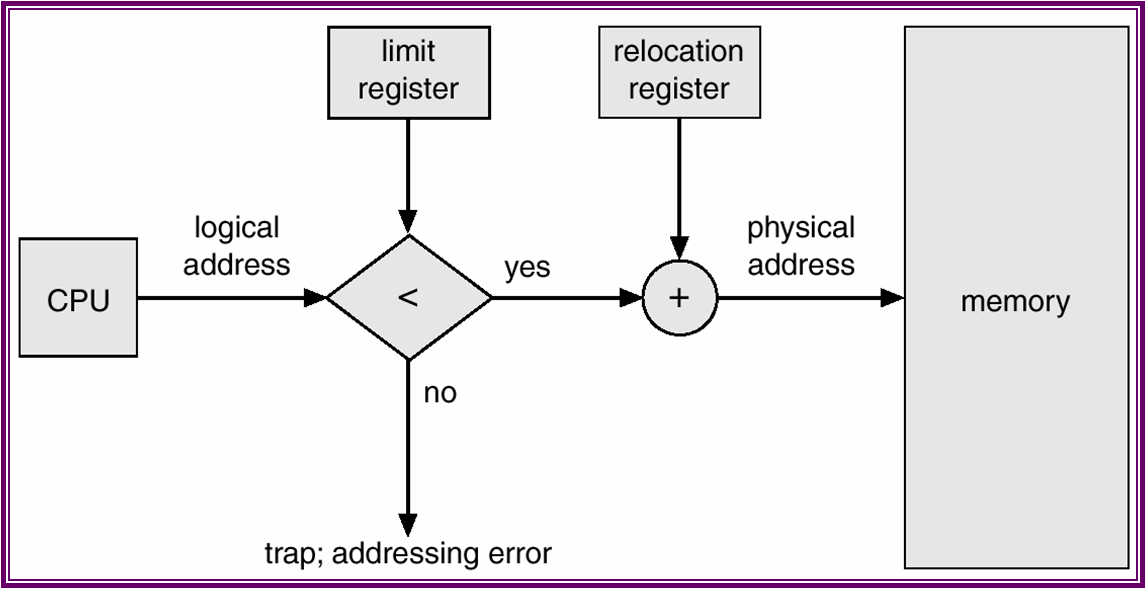
\includegraphics[scale=0.5]{v6f9-5}
  \end{center}
  \end{frame}
  
  %% PAGE
  \begin{frame}
  \frametitle{Protection: 总结} \pause
  \begin{itemize}
  \item{内存保护是现代操作系统必备的功能之一,} \pause
    \begin{itemize}
    \item{它需要硬件的支持才能实施保护。} \pause
    \end{itemize}
  \item{后面讲解的各种内存管理方法都包含有内存保护的方法。}
  \end{itemize}
  \end{frame}
  
  %% PAGE
  \begin{frame}
  \frametitle{Questions}
  \begin{itemize}
  \item{Any questions?}
  \end{itemize}
  \begin{center}
    
\includegraphics[scale=.5]{question}
  \end{center}
  \end{frame}

  %% PAGE
  \begin{frame}
  \frametitle{Allocation: 问题} \pause
  \begin{itemize}
  \item{在多任务的环境中,} \pause
    \begin{itemize}
    \item{操作系统需要为每个新创建的进程分配一定数量的内存才能运行;} \pause
    \item{当进程退出时,操作系统要回收它所占用的内存。} \pause
    \end{itemize}
  \item{问题:} \pause
    \begin{itemize}
    \item{操作系统如何有效地管理内存的分配和回收,以尽量满足进程的需求?} \pause
    \item{这个问题也称为动态内存分配问题(Dynamic memory allocation problem)。}
    \end{itemize}
  \end{itemize}
  \end{frame}
  
  %% PAGE
  \begin{frame}
  \frametitle{Allocation: How to do?} \pause
  \begin{itemize}
  \item{The OS keeps a table indicating which parts of memory are available and which are occupied.} \pause
    \begin{itemize}
    \item{Available memory blocks are called \textbf{holes}.} \pause
    \item{Initially, all memory is available for user processes.} \pause
    \item{When a process arrives and needs memory, OS search for a hole large enough for it.} \pause
    \item{When a process terminates, it returns the memory to OS as a hole, and} \pause
    \item{If the new hole is adjacent(相邻) to other holes, these adjacent holes are merged(合并) to form one larger hole.}
    \end{itemize}
  \end{itemize}
  \end{frame}
  
  %% PAGE
  \begin{frame}
  \frametitle{Allocation: Example} \pause
  \setlength{\unitlength}{.5cm}
  \begin{picture}(22, 15)
    \put(1, 0){Initially}
    \put(0, 1){\framebox(4, 4){OS kernel}}
    \put(0, 5){\framebox(4, 10){hole}} \pause

    \put(6, 0){A enters}
    \put(5, 1){\framebox(4, 4){OS kernel}}
    \put(5, 5){\framebox(4, 2){A}}
    \put(5, 7){\framebox(4, 8){hole}} \pause

    \put(11, 0){B enters}
    \put(10, 1){\framebox(4, 4){OS kernel}}
    \put(10, 5){\framebox(4, 2){A}}
    \put(10, 7){\framebox(4, 3){B}}
    \put(10, 10){\framebox(4, 5){hole}} \pause

    \put(16, 0){A leaves}
    \put(15, 1){\framebox(4, 4){OS kernel}}
    \put(15, 5){\framebox(4, 2){hole}}
    \put(15, 7){\framebox(4, 3){B}}
    \put(15, 10){\framebox(4, 5){hole}} \pause

    \put(20, 0){Going on}
    \put(20.5, 8){......}
  \end{picture}
  \end{frame}
  
  %% PAGE
  \begin{frame}
  \frametitle{Allocation: 算法} \pause
  \begin{itemize}
  \item{随着系统中进程的创建和退出,系统中的内存可能会形成很多小的hole,} \pause
    \begin{itemize}
    \item{这些hole既不足以满足任何的进程需求,也不能被合并以形成大的hole。这些hole被称为外部碎片(external fragmentation)。} \pause
    \end{itemize}
  \item{因此,必须设计出专门算法来进行内存的分配和释放以减少外部碎片,提高内存使用率。简单、常用的有:} \pause
    \begin{itemize}
    \item{首次适应(First fit):Allocate the first hole that is big enough.} \pause
    \item{最佳适应(Best fit):Allocate the smallest hole that is big enough.} \pause
    \item{最坏适应(Worst fit):Allocate the largest hole.}
    \end{itemize}
  \end{itemize}
  \end{frame}
  
  %% PAGE
  \begin{frame}
  \frametitle{Allocation: 另一种方法} \pause
  \begin{minipage}[c]{0.6\textwidth}
    \begin{itemize}
    \item{我们把系统内存分成固定大小的内存块,} \pause
      \begin{itemize}
      \item{操作系统以块为单位进行内存的分配和释放。} \pause
      \item{最终分配给进程的内存可能会比所请求要多一点,如右图所示。} \pause
      \item{我们称这多出来的部分为内部碎片(Internal Fragmentation)。} \pause
      \end{itemize}
    \end{itemize}
  \end{minipage}%
  \begin{minipage}[c]{0.4\textwidth}
    \setlength{\unitlength}{.5cm}
    \begin{picture}(5, 15)
      \put(1, 0){\framebox(5, 3){OS kernel}}
      \multiput(1, 3)(0, 1){8}{\framebox(5, 1){}}
      \color{blue}
      \put(0.9,2.9){\framebox(5.2, 3.2){}}
      \put(7, 4.1){A}
      \color{red}
      \tiny
      \put(1,5.5){\framebox(5, 0.5){internal fragmentation}}      
    \end{picture}
  \end{minipage}
  \end{frame}
  
  %% PAGE
  \begin{frame}
  \frametitle{Allocation: 总结(1/2)} \pause
  \begin{itemize}
  \item{Allocation主要解决在多任务的环境中,操作系统采用什么算法进行内存的分配和回收,减少外部碎片或内部碎片,提高内存利用率。} \pause
    \begin{itemize}
    \item{相对于外部碎片,内部碎片的情况不是很严重;} \pause
    \item{后面我们将介绍两种消除外部碎片的方法。}
    \end{itemize}
  \end{itemize}
  \end{frame}
  
  %% PAGE
  \begin{frame}
  \frametitle{Allocation: 总结(2/2)}
  \begin{minipage}[c]{0.7\textwidth} \pause
    \begin{itemize}
    \item{事实上,内存的分配和回收问题不仅出现在OS中,应用程序面临着同样的问题。} \pause
      \begin{itemize}
      \item{当进程被创建时,操作系统会采用某种算法分配一块足够大的内存给进程,由进程自己管理(其中的一部分),如图所示:} \pause
      \end{itemize}
    \item{在该图中,} \pause
      \begin{itemize}
      \item{\textbf{heap}由进程自己管理。库函数new/delete(或malloc/free)就是操纵heap中的内存。它们所采用的分配与回收算法非常通用,相应的空间和时间利用率也很一般。在一个大型的项目中,已有的库函数可能不会满足应用的要求,需要自己开发更好的来替换它们以负责heap中内存的分配与回收。} \pause
      \end{itemize}
    \end{itemize}
  \end{minipage}%
  \begin{minipage}[c]{0.3\textwidth}
    \setlength{\unitlength}{.5cm}
    \centering
    \begin{picture}(5, 15)
      \put(1, 0){\framebox(5, 2){code}}
      \put(1, 2){\framebox(5, 2){data}}
      \put(1, 4){\framebox(5, 3){heap}}
      \put(1, 7){\framebox(5, 2){free}}
      \put(1, 9){\framebox(5, 2){stack}}
      \put(5, 6){\vector(0, 1){2}}
      \put(2, 10){\vector(0, -1){2}}
    \end{picture}
%    \newline 进程在内存中的镜像(Process image) \pause
  \end{minipage}
  \end{frame}
  
  %% PAGE
  \begin{frame}
  \frametitle{Questions}
  \begin{itemize}
  \item{Any questions?}
  \end{itemize}
  \begin{center}
    
\includegraphics[scale=.5]{question}
  \end{center}
  \end{frame}
  
\section{分页内存管理}

  %% PAGE
  \begin{frame}
  \frametitle{介绍(1/2)} \pause
  \begin{itemize}
  \item{基本内存管理方法存在着很大的限制,} \pause
    \begin{itemize}
    \item{每个进程所占用的物理内存必须是连续的,} \pause
    \item{系统可能会产生大量的外部碎片,最后不可避免地要进行compaction,} \pause
    \item{对整个进程进行swap-in/swap-out非常地耗时。} \pause
    \end{itemize}
  \item{分页很好地解决了上面的问题,} \pause
    \begin{itemize}
    \item{进程所占用的物理内存不必连续,} \pause
    \item{没有外部碎片,但是会有一定量的内部碎片,} \pause
    \item{对进程所占用的部分内存进行swap-in/swapout。} \pause
    \end{itemize}
  \item{在早期,分页系统主要由硬件来实现;如今,分页由硬件和操作系统共同完成。}
  \end{itemize}
  \end{frame}
  
  %% PAGE
  \begin{frame}
  \frametitle{介绍(2/2)} \pause
  \begin{itemize}
  \item{基本概念} \pause
    \begin{itemize}
    \item{Physical memory is broken into fixed-sized blocks called \textbf{frames}.} \pause
    \item{Logical memory is also broken into blocks of the same size called \textbf{pages}.} \pause
    \item{\textbf{Page tables} are used to map pages to frames.} \pause
      \begin{itemize}
      \item{An entry of the page table is called \textbf{Page Table Entry (PTE).}}
      \end{itemize}
    \end{itemize}
  \end{itemize}
  \end{frame}
  
  %% PAGE
  \begin{frame}
  \frametitle{方法} \pause
  \begin{itemize}
  \item{把逻辑地址分成两部分:} \pause
    \begin{itemize}
    \item{第一部分称为\textbf{page number};} \pause
    \item{第二部分称为\textbf{page offset}。} \pause
    \end{itemize}
  \item{地址转换} \pause
    \begin{itemize}
    \item{在page table的帮助下,MMU把CPU产生的逻辑地址转换成物理地址。}
    \end{itemize}
  \end{itemize}
  \end{frame}
  
  %% PAGE
  \begin{frame}
  \frametitle{过程} \pause
  \begin{center}
    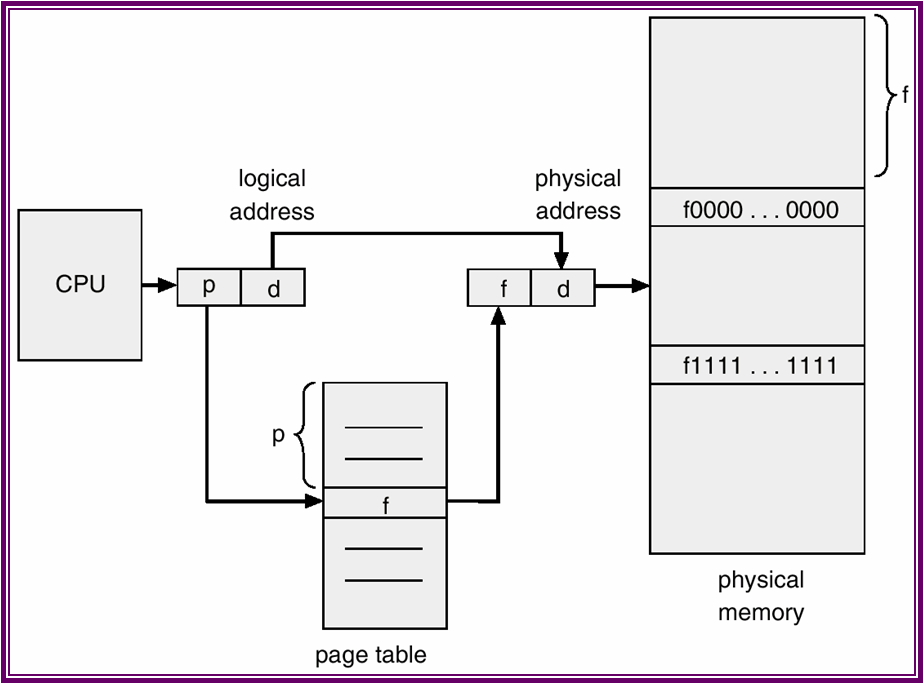
\includegraphics[scale=.6]{v6f9-6}
  \end{center}
  \end{frame}
  
  %% PAGE
  \begin{frame}
  \frametitle{例子(1/2)} \pause
  \begin{center}
    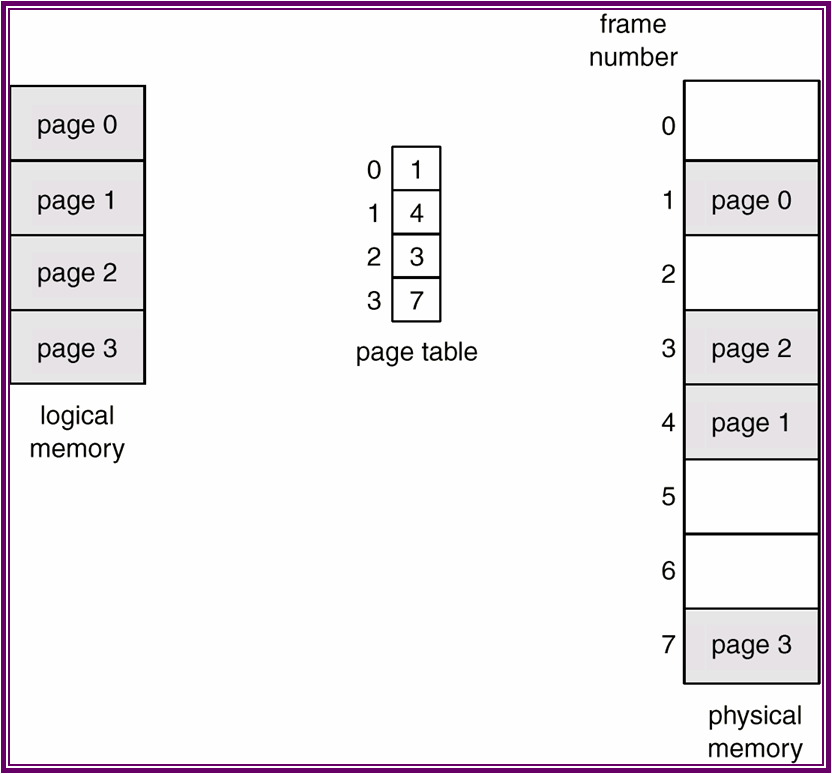
\includegraphics[scale=.5]{v6f9-7}
  \end{center}
  \end{frame}
  
  %% PAGE
  \begin{frame}
  \frametitle{例子(2/2)} \pause
  \begin{center}
    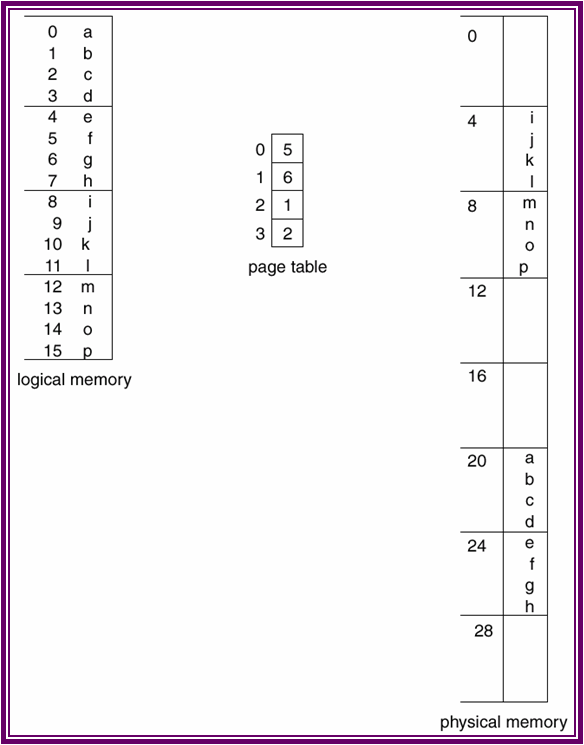
\includegraphics[scale=.6]{v6f9-8}
  \end{center}
  \end{frame}
  
  %% PAGE
  \begin{frame}
    \frametitle{地址划分} \pause
    \begin{itemize}
    \item{page和frame:} \pause
      \begin{itemize}
      \item{它们的大小必须相同,都是2的幂次方;} \pause
      \item{具体由CPU体系结构决定,常见的有1K、4K、8K、4M等。} \pause
      \end{itemize}
    \item{地址划分} \pause
      \begin{itemize}
      \item{如果逻辑地址空间的大小为$2^m$,而page或frame的大小为$2^n$($n<m$),那么逻辑地址的划分如图所示:} \pause
      \end{itemize}
    \end{itemize}
    \begin{center}
      \setlength{\unitlength}{.5cm}
      \begin{picture}(15, 5)
        \put(1, 1){\framebox(6, 2){page number}}
        \put(7, 1){\framebox(6, 2){page offset}}
        \put(10, 0){n}
        \put(4, 0){m-n}
        \put(13, 3){0}
        \put(0, 3){m-1}
      \end{picture}
    \end{center}
  \end{frame}
  
  %% PAGE
  \begin{frame}
  \frametitle{结论} \pause
  \begin{itemize}
  \item{An important aspect of paging is the clear separation between user's view of memory and the actual physical memory, } \pause
    \begin{itemize}
    \item{The difference them is reconciled by address translation hardware;} \pause
    \item{This mapping is hidden from the user and is controlled by the OS.} \pause
    \end{itemize}
  \item{由于是操作系统在控制地址映射,它必须} \pause
    \begin{itemize}
    \item{记录系统物理内存的使用状况。一般使用一个称为frame table的数据结构来保存系统中每一个frame的状态;} \pause
    \item{为每一个进程保存一个page table。}
    \end{itemize}
  \end{itemize}
  \end{frame}
  
  %% PAGE
  \begin{frame}
  \frametitle{Questions}
  \begin{itemize}
  \item{Any questions?}
  \end{itemize}
  \begin{center}
    
\includegraphics[scale=.5]{question}
  \end{center}
  \end{frame}
  
  %% PAGE
  \begin{frame}
  \frametitle{实现} \pause
  \begin{itemize}
  \item{Page table必须被保存在内存中。CPU中的两个寄存器记录了它的信息:}  \pause
    \begin{itemize}
    \item{\textbf{Page-table base register (PTBR)} 保存了page table的地址;} \pause
    \item{\textbf{Page-table length register (PTLR)} 保存了page table的大小。} \pause
    \end{itemize}
  \item{因此在分页中,每一个内存访问都需要两次内存操作,} \pause
    \begin{itemize}
    \item{一次访问page table,一次访问内存数据。} \pause
    \item{考虑到CPU访问内存的频率,这种地址转换成了系统性能的颈瓶。} \pause
    \end{itemize}
  \item{为了提高地址转换效率,MMU中包含了一个高速缓存称为\textbf{translation look-aside buffers(TLBs)} 。}
  \end{itemize}
  \end{frame}

  %% PAGE
  \begin{frame}
  \frametitle{TLB} \pause
  \begin{itemize}
  \item{TLB结构如图所示:} \pause
  \end{itemize}
  \setlength{\unitlength}{.5cm}
  \centering
  \begin{picture}(15, 6)
    \multiput(1, 1)(0, 1){4}{\framebox(6, 1){}}
    \multiput(7, 1)(0, 1){4}{\framebox(6, 1){}}
    \put(3, 5.5){Page \#}
    \put(9, 5.5){Frame \#}
    \put(6.5, 0){TLB} \pause
  \end{picture}
  \begin{itemize}
  \item{Address translation of \emph{A}, } \pause
    \begin{itemize}
    \item{If \emph{A} is in TLB (TLB hit), get frame \# out;} \pause
    \item{Otherwise, get frame \# from the page table in the memory.}
    \end{itemize}
  \end{itemize}
  \end{frame}
  
  %% PAGE
  \begin{frame}
    \frametitle{Address translation with TLB} \pause
    \begin{center}
      \setlength{\unitlength}{.5cm}
      \begin{picture}(15, 15)
        \color{red}
        \put(0, 0){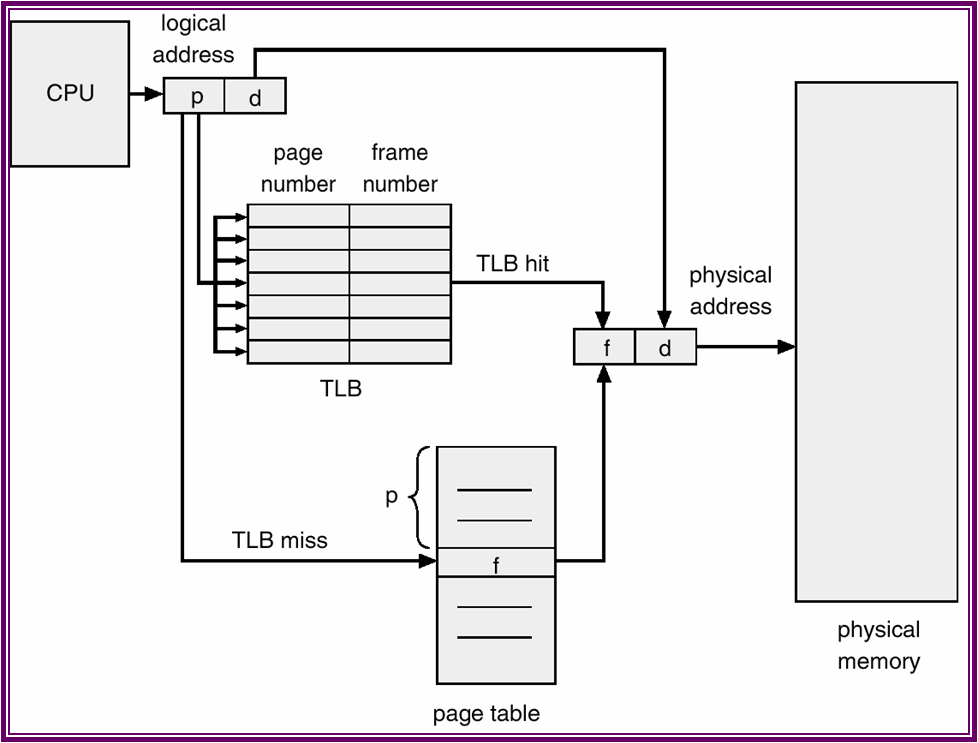
\includegraphics[scale=.5]{v6f9-10}} \pause
        \put(2.5, 5.5){\framebox(10, 5){}}
        \put(0.5, 7.5){MMU}
      \end{picture}
    \end{center}
  \end{frame}
  
  %% PAGE
  \begin{frame}
  \frametitle{性能} \pause
  \begin{itemize}
  \item{假设} \pause
    \begin{itemize}
    \item{TLB lookup time = $\epsilon$, } \pause
    \item{Memory cycle time is 1 microsecond ($10^{-6}$ second),} \pause
    \item{TLB hit ratio $=\alpha$, percentage of times that a page number is found in the TLB.} \pause
    \end{itemize}
  \item{Effective Access Time (EAT)} \pause
    \begin{itemize}
    \item{$EAT=(1+\epsilon)\alpha+(2+\epsilon)(1-\alpha) = 2+\epsilon-\alpha$}
    \end{itemize}
  \end{itemize}
  \end{frame}
  
  %% PAGE
  \begin{frame}
  \frametitle{内存保护} \pause
  \begin{itemize}
  \item{在分页系统中,内存保护是以页为单位。} \pause
    \begin{itemize}
    \item{保护信息通常都保存在PTE中,} \pause
    \item{可以提供只读、读写和执行(RWX - Read, Write, eXecute)保护。} \pause
    \end{itemize}
  \item{此外,不是所有的PTE都可以使用。因此,PTE中的一位表示该PTE是否可以使用(valid/invalid),} \pause
    \begin{itemize}
    \item{仅当该位有效时,MMU才能用它进行地址转换,} \pause
    \item{否则,MMU将通过异常向OS报告错误。}
    \end{itemize}
  \end{itemize}
  \end{frame}
  
  %% PAGE
  \begin{frame}
    \frametitle{例子}
    \begin{center}
      \setlength{\unitlength}{.5cm}
      \begin{picture}(15, 15)
        % \color{red}
        \put(0, 0){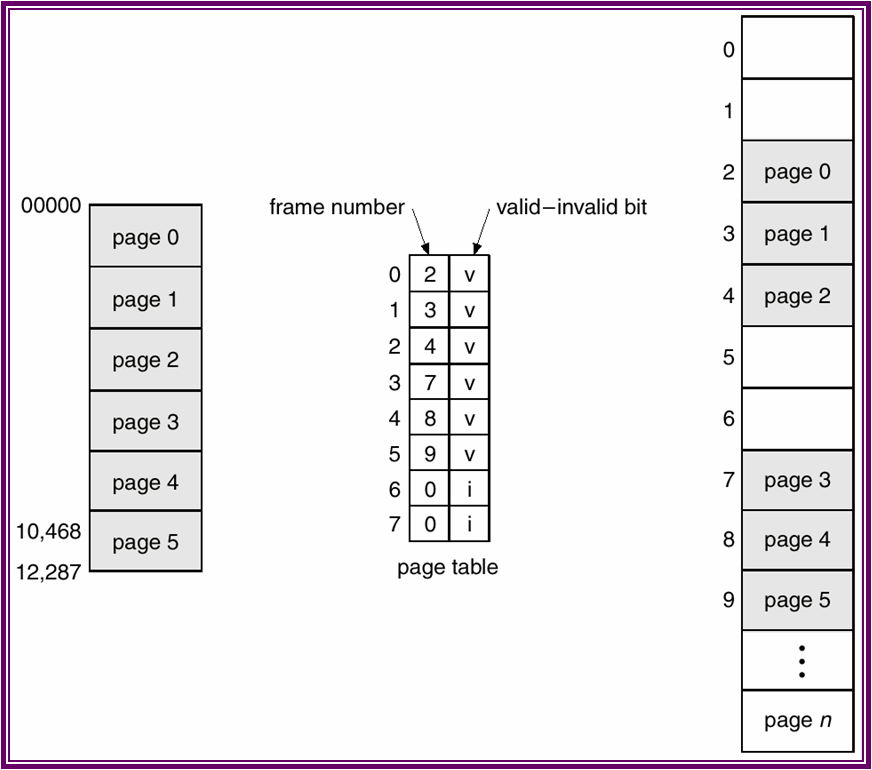
\includegraphics[scale=.6]{v6f9-11}}
        \put(9.95, 4.68){\framebox(1, 5.8){\tiny{RWX}}}
      \end{picture}
    \end{center}
  \end{frame}
  
  %% PAGE
  \begin{frame}
  \frametitle{Questions}
  \begin{itemize}
  \item{Any questions?}
  \end{itemize}
  \begin{center}
    
\includegraphics[scale=.5]{question}
  \end{center}
  \end{frame}
  
  %% PAGE
  \begin{frame}
  \frametitle{页表问题} \pause
  \begin{itemize}
  \item{假设} \pause
    \begin{itemize}
    \item{逻辑地址空间大小:$2^{32}$,即4GB;} \pause
    \item{page和frame的大小:$2^{12}$,即4KB;} \pause
    \item{sizeof(PTE) = 4B。} \pause
    \end{itemize}
  \item{一个页表要消耗多少内存?} \pause
    \begin{itemize}
    \item{$\frac{2^{32}}{2^{12}}\times4 = 4MB$.} \pause
    \end{itemize}
  \item{记住:每一个进程都需要一个页表,} \pause
    \begin{itemize}
    \item{一个只有256MB内存的系统如何能同时运行几十个进程呢?}
    \end{itemize}
  \end{itemize}
  \end{frame}
  
  %% PAGE
  \begin{frame}
  \frametitle{页表结构} \pause
  \begin{itemize}
  \item{事实上,很少的进程会使用整个地址空间(如32位机器上的4GB和64位机器上的$2^{64}B$);} \pause
    \begin{itemize}
    \item{也就是说,页表中大部分的PTE都是处于invalid状态。但是,} \pause
    \item{OS无法预测一个进程的页表大小,因此只能根据进程使用内存的情况动态地伸缩。} \pause
    \item{显然线性的页表结构太简单,不能满足这个要求,我们需要新的页表结构。} \pause
    \end{itemize}
  \item{现有的页表结构:} \pause
    \begin{itemize}
    \item{Hierarchical Page Tables} \pause
    \item{Hashed Page Tables} \pause
    \item{Inverted Page Tables}
    \end{itemize}
  \end{itemize}
  \end{frame}
  
  %% PAGE
  \begin{frame}
  \frametitle{Hierarchical Page Tables(层次型页表)} \pause
  \begin{itemize}
  \item{这种方法采用“树”结构来组织页表,形成一个层次结构的页表;} \pause
    \begin{itemize}
    \item{根据这颗树的深度可以分为:一、二、三级页表等;\pause其中,一级页表(也称为单级页表)就退化成了线性页表。} \pause
    \item{这里以32位逻辑地址、页面大小为4KB为例来讲解二级页表。}
    \end{itemize}
  \end{itemize}
  \end{frame}
  
  %% PAGE
  \begin{frame}
  \frametitle{二级页表设计} \pause
  \begin{itemize}
  \item{Paging the page table} \pause
    \begin{itemize}
    \item{把一个巨大的线性页表分割成很多小的页表:} \pause
      \begin{itemize}
      \item{每一个小页表包含1024项PTE,\pause因此需要1024个小页表才能覆盖4GB的地址空间;} \pause
      \item{又sizeof(PTE)=4B,所以一个小页表恰好占4KB,即一个页面。} \pause
      \end{itemize}
    \item{然后通过一个称为outer page table的表把这些小页表组织起来。} \pause
      \begin{itemize}
      \item{显然,outer page table中包含1024项指向小页表的指针。} \pause
      \item{通常称outer page table为\textbf{page directory},其中的每一项称为\textbf{Page Directory Entry(PDE)。}} \pause
      \item{由于sizeof(\color{red}\textbf{PDE}\normalcolor)=4B,所以page directory也占4KB,即一个页面。}
      \end{itemize}
    \end{itemize}
  \end{itemize}
  \end{frame}
  
  %% PAGE
  \begin{frame}
  \frametitle{二级页表结构} \pause
  \begin{center}
    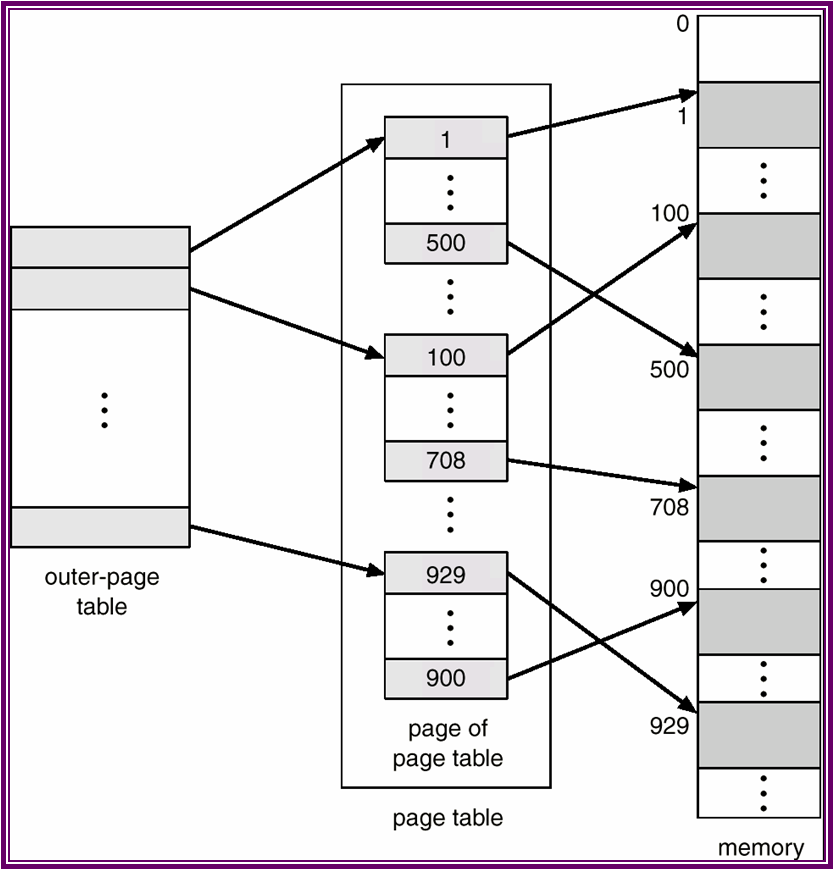
\includegraphics[scale=.5]{v6f9-12}
  \end{center}
  \end{frame}
  
  %% PAGE
  \begin{frame}
  \frametitle{地址划分} \pause
  \begin{itemize}
  \item{Remember that in single level page tables, a logical address is divided into:} \pause
    \begin{itemize}
    \item{a page number consisting of 20 bits,} \pause
    \item{a page offset consisting of 12 bits.} \pause
    \end{itemize}
  \item{Now since the page table is paged, the page number is further divided into:} \pause
    \begin{itemize}
    \item{a 10-bit page number,} \pause
    \item{a 10-bit page offset.} \pause
    \end{itemize}
  \end{itemize}
  \setlength{\unitlength}{.5cm}
  \centering
  \begin{picture}(20, 6)
    % \color{red}
    \put(11, 6){page number}
    \put(18, 6){page offset}

    \put(-1, 4){采用一级页表的逻辑地址:}
    \put(9, 3.8){\framebox(8, 1){p}}
    \put(17, 3.8){\framebox(4.8, 1){d}}
    \put(12.5, 3.2){20}
    \put(18.9, 3.2){12} \pause

    \put(-1, 1){采用二级页表的逻辑地址:}
    \put(9, 0.8){\framebox(4, 1){$p_{1}$}}
    \put(13, 0.8){\framebox(4, 1){$p_{2}$}}
    \put(17, 0.8){\framebox(4.8, 1){d}}
    \put(10.5, 0.2){10}
    \put(14.5, 0.2){10}
    \put(18.9, 0.2){12}
  \end{picture}
  \end{frame}
  
  %% PAGE
  \begin{frame}
    \frametitle{地址转换} \pause
    \begin{center}
      \setlength{\unitlength}{.5cm}
      \begin{picture}(20, 16)
        \put(0, 7){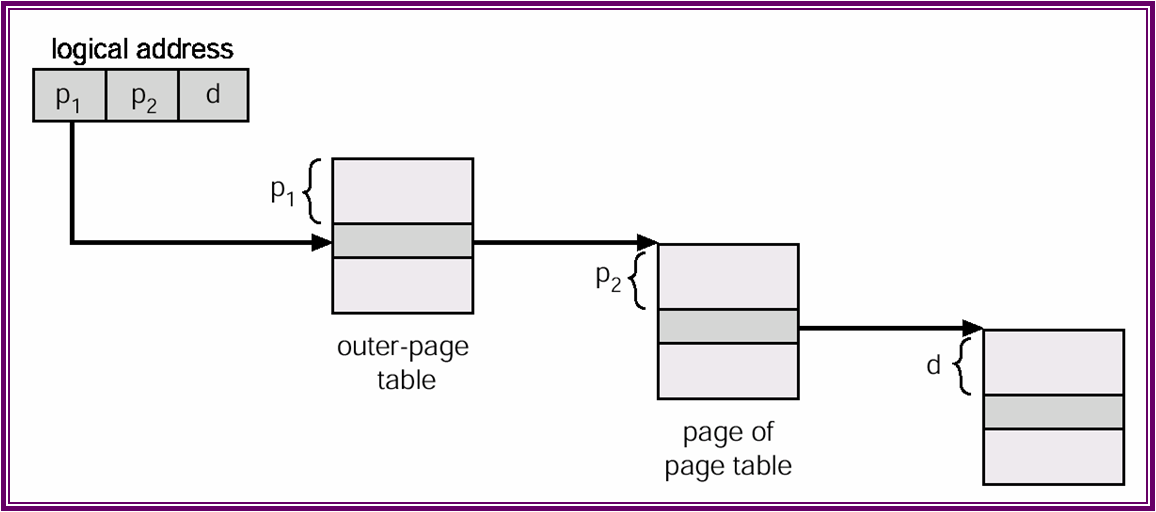
\includegraphics[scale=.5]{v6f9-13}}
        \put(15.8, 14.7){\tiny{physical address}}
        \put(15, 13.8){\framebox(3, 0.8){f}}
        \put(18, 13.8){\framebox(1.2, 0.8){d}}
      \end{picture}
    \end{center}
  \end{frame}
  
  %% PAGE
  \begin{frame}
  \frametitle{例子(1/3)} \pause
  \begin{itemize}
  \item{Intel IA-32(x86,i386)中的PTE:} \pause
  \end{itemize}
  \begin{center}
    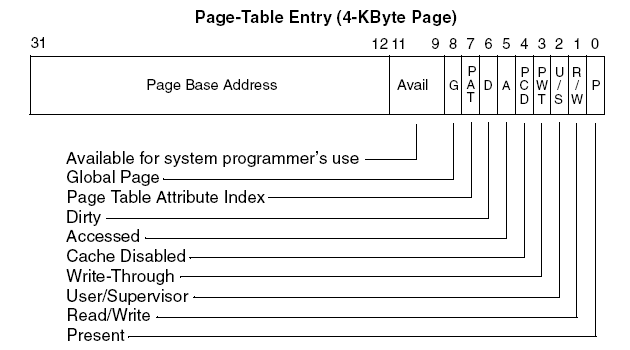
\includegraphics[scale=.5]{x86pte} \pause
  \end{center}
  \begin{itemize}
  \item{其中的“Present”为就是前面讲到的valid/invalid位。}
  \end{itemize}
  \end{frame}
  
  %% PAGE
  \begin{frame}
  \frametitle{例子(2/3)} \pause
  \begin{itemize}
  \item{Intel IA-32(x86,i386)中的PDE:} \pause
  \end{itemize}
  \begin{center}
    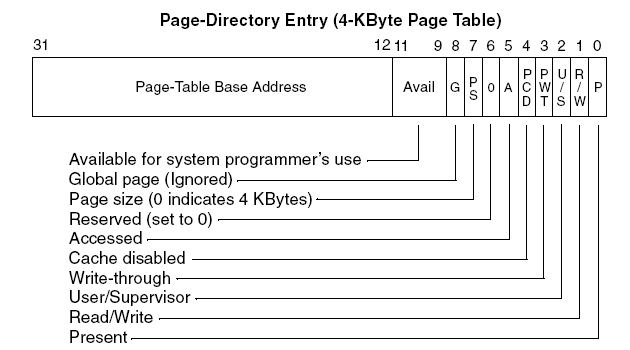
\includegraphics[scale=.5]{x86pde} \pause
  \end{center}
  \begin{itemize}
  \item{其中的“Present”为就是前面讲到的valid/invalid位。}
  \end{itemize}
  \end{frame}
  
  %% PAGE
  \begin{frame}
  \frametitle{例子(3/3)} \pause
  \begin{itemize}
  \item{Intel IA-32(x86,i386)中的地址转换:} \pause
  \end{itemize}
  \begin{center}
    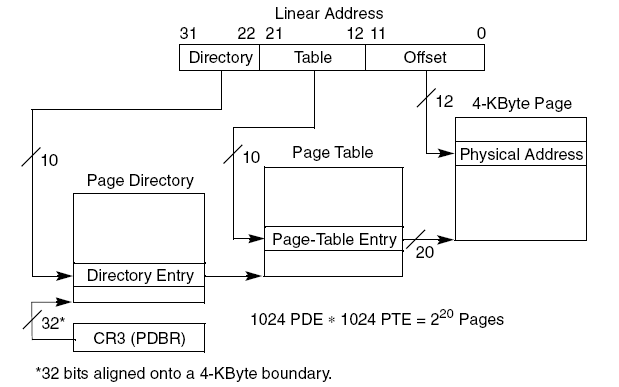
\includegraphics[scale=0.5]{x86atl2p} \pause
  \end{center}
  \begin{itemize}
  \item{其中的“PDBR”全称为Page Directory Base Register。}
  \end{itemize}
  \end{frame}
  
  %% PAGE
  \begin{frame}
  \frametitle{Questions}
  \begin{itemize}
  \item{Any questions?}
  \end{itemize}
  \begin{center}
    
\includegraphics[scale=.5]{question}
  \end{center}
  \end{frame}
  
\iffalse

  %% PAGE
  \begin{frame}
  \frametitle{Hashed Page Tables} \pause
  \begin{itemize}
  \item{Common in address spaces $>$ 32 bits.} \pause
  \item{The virtual page number is hashed into a page table.} \pause
    \begin{itemize}
    \item{This page table contains a chain of elements hashing to the same location.} \pause
    \end{itemize}
  \item{Virtual page numbers are compared in this chain searching for a match.} \pause
    \begin{itemize}
    \item{If a match is found, the corresponding physical frame is extracted.}
    \end{itemize}
  \end{itemize}
  \end{frame}
  
  %% PAGE
  \begin{frame}
  \frametitle{Hashed Page Table Architecture} \pause
  \begin{center}
    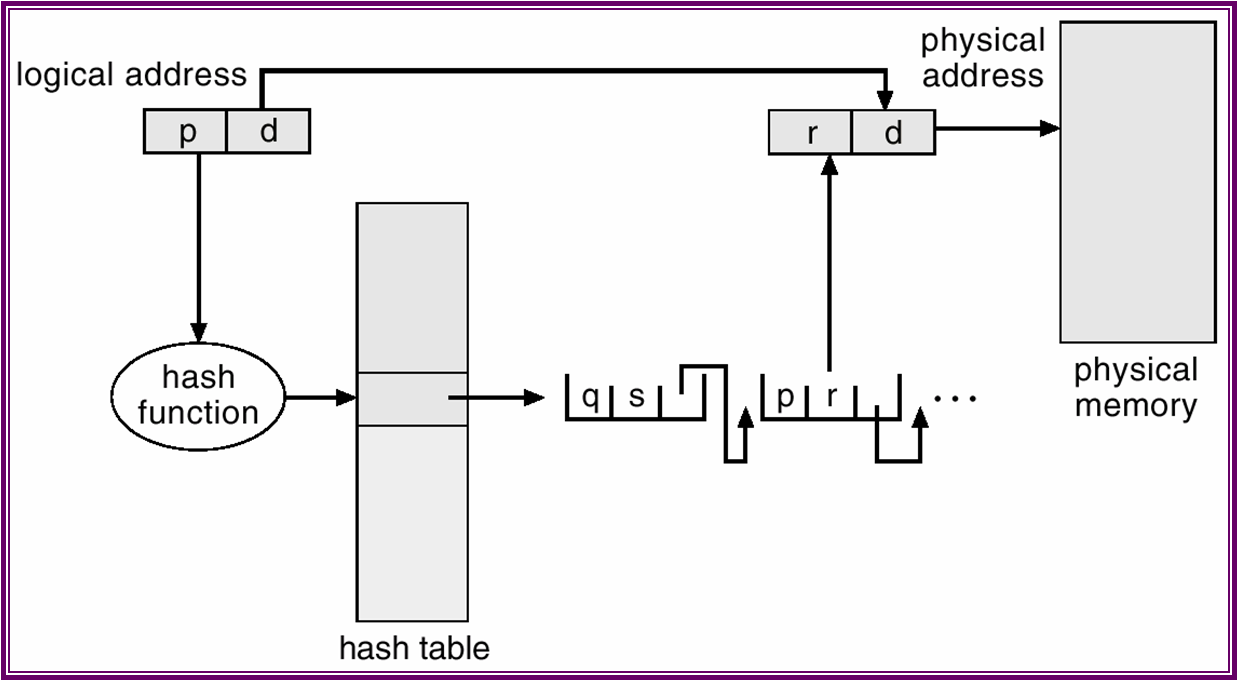
\includegraphics[scale=.5]{v6f9-14}
  \end{center}
  \end{frame}
  
  %% PAGE
  \begin{frame}
  \frametitle{Questions}
  \begin{itemize}
  \item{Any questions?}
  \end{itemize}
  \begin{center}
    
\includegraphics[scale=.5]{question}
  \end{center}
  \end{frame}
  
  %% PAGE
  \begin{frame}
  \frametitle{Inverted Page Tables} \pause
  \begin{itemize}
  \item{Common in address spaces $>$ 32 bits, too.} \pause
  \item{One entry for each frame of memory.} \pause
    \begin{itemize}
    \item{Entry consists of the virtual address of the page stored in that real memory location, with information about the process that owns that page.} \pause
    \end{itemize}
  \item{Decreases memory needed to store each page table, but increases time needed to search the table when a page reference occurs.} \pause
    \begin{itemize}
    \item{Use hash table to limit the search to one — or at most a few — page-table entries.}
    \end{itemize}
  \end{itemize}
  \end{frame}
  
  %% PAGE
  \begin{frame}
  \frametitle{Inverted Page Table Architecture} \pause
  \begin{center}
    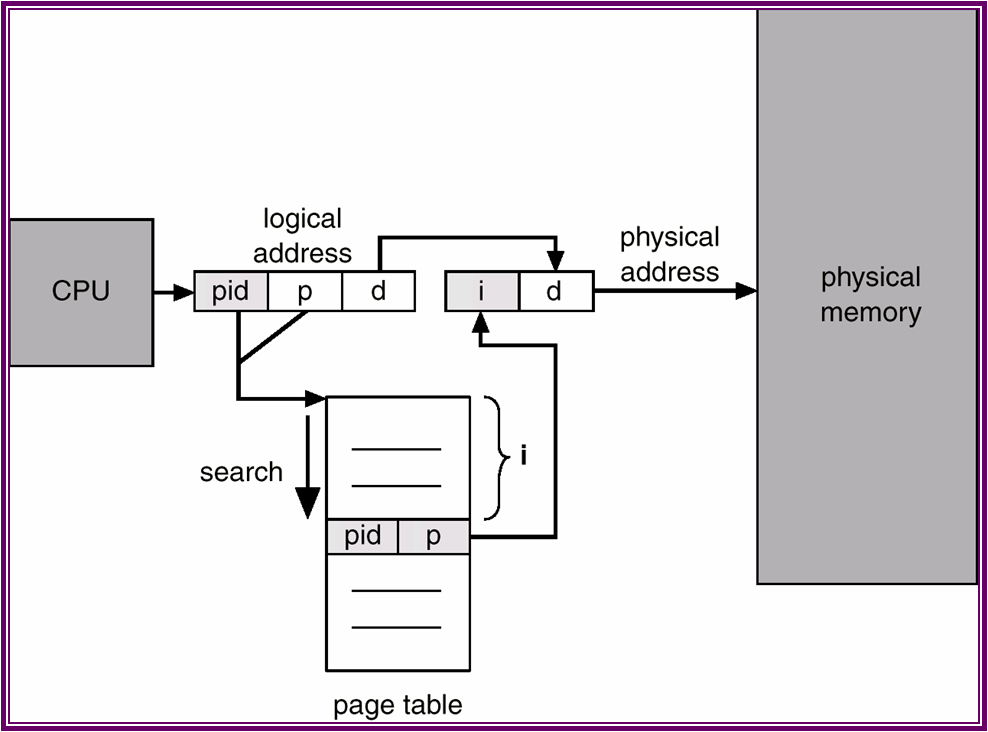
\includegraphics[scale=.5]{v6f9-15}
  \end{center}
  \end{frame}
  
  %% PAGE
  \begin{frame}
  \frametitle{Questions}
  \begin{itemize}
  \item{Any questions?}
  \end{itemize}
  \begin{center}
    
\includegraphics[scale=.5]{question}
  \end{center}
  \end{frame}
  
\fi

  %% PAGE
  \begin{frame}
  \frametitle{Frame management(1/2)} \pause
  \begin{itemize}
  \item{前面介绍了页面的管理,以及页面到frame的映射。} \pause
    \begin{itemize}
    \item{但是,最终保存数据的地方是frame,而不是页面。} \pause
    \end{itemize}
  \item{操作系统需要管理系统中所有frame的分配和回收,} \pause
    \begin{itemize}
    \item{当进程被创建时,操作系统要分配足够多的frame给它,并在该进程的页表中做相应的映射;} \pause
    \item{当进程退出时,操作系统回收它所占用的frame。}
    \end{itemize}
  \end{itemize}
  \end{frame}
  
  %% PAGE
  \begin{frame}
  \frametitle{Frame management(2/2)} \pause
  \begin{itemize}
  \item{最简单的方法是维护一个空闲的frame链表(free-frame list),如图所示:} \pause
  \end{itemize}
  \begin{center}
    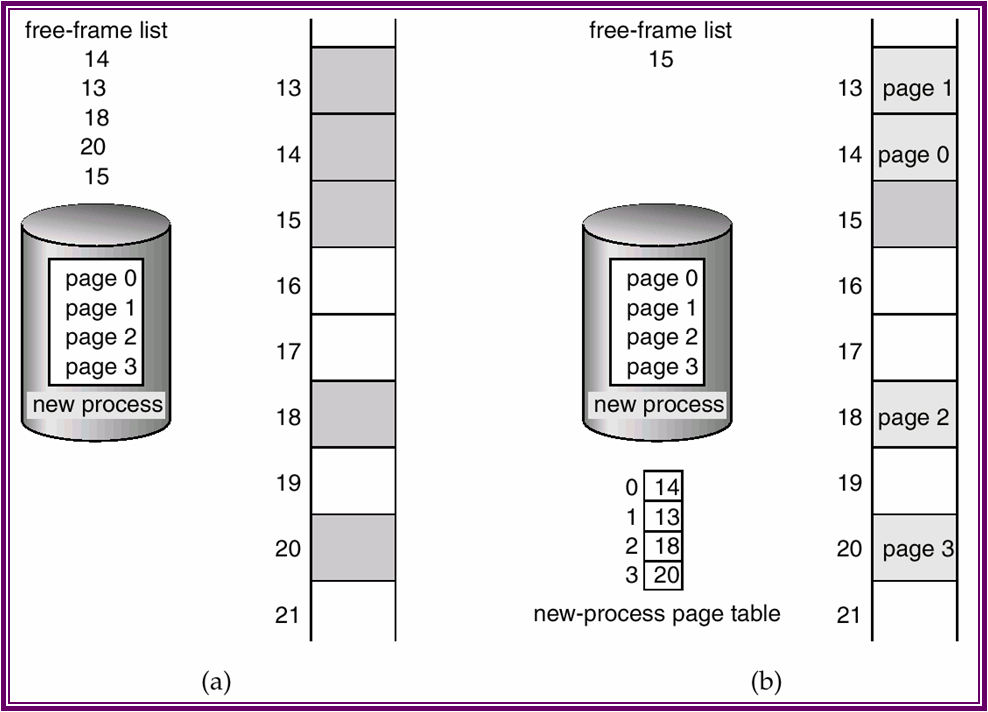
\includegraphics[scale=.5]{v6f9-9}
  \end{center}
  \end{frame}
  
  %% PAGE
  \begin{frame}
  \frametitle{Questions}
  \begin{itemize}
  \item{Any questions?}
  \end{itemize}
  \begin{center}
    
\includegraphics[scale=.5]{question}
  \end{center}
  \end{frame}
  

  %% PAGE
  \begin{frame}
  \frametitle{页面共享} \pause
  \renewcommand{\thefootnote}{\fnsymbol{footnote}}
  \begin{itemize}
  \item{在分页系统中,显然应该以页面为单位进行内存共享。} \pause
    %\begin{itemize}
    %\item{如果某一个或几个页面包含所谓的纯代码(pure code),也就是可重入代码(reentrant code)。} \pause
    %\item{每个进程只要把这些页面通过自己的页表映射到自己的地址空间里来即可。}
    %\end{itemize}
  \item{例子} \pause
    \begin{itemize}
    \item{假设系统中有三个用户同时运行某个编辑器在编辑各自的文件,显然编辑器的代码可以被共享,而各自的文件数据则是私有的。} \pause
    \end{itemize}
  \end{itemize}
  \begin{center}
  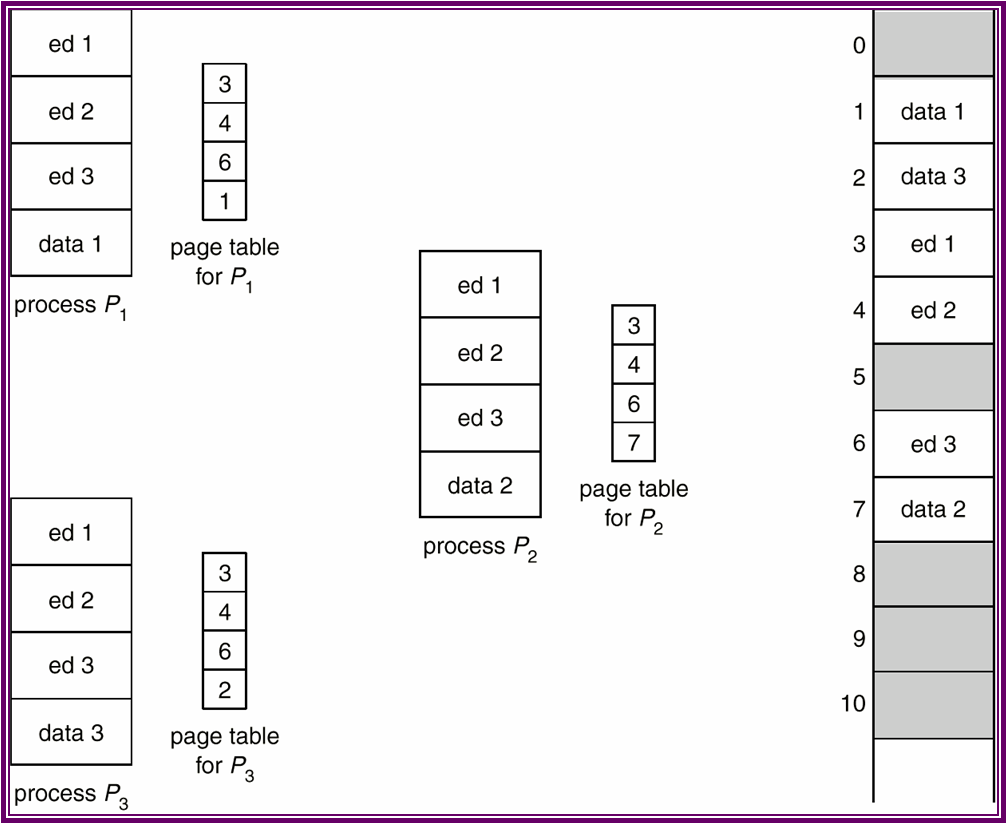
\includegraphics[scale=.3]{v6f9-16}
  \end{center}
  %\renewcommand{\thefootnote}{\arabic{footnote}}
  \end{frame}
  
  %% PAGE
  \begin{frame}
  \frametitle{Questions}
  \begin{itemize}
  \item{Any questions?}
  \end{itemize}
  \begin{center}
    
\includegraphics[scale=.5]{question}
  \end{center}
  \end{frame}

\section{分段内存管理}  
  
  %% PAGE
  \begin{frame}
  \frametitle{介绍} \pause
  \begin{itemize}
  \item{Why segmentation?} \pause
    \begin{itemize}
    \item{Usually, users do not think of memory as a linear array of bytes or pages, some containing instructions and others contains data.} \pause
    \item{Rather, users prefer to view memory as a collection of variable-sized segments.} \pause
    \end{itemize}
  \item{什么是分段?} \pause
    \begin{itemize}
    \item{分段把进程的逻辑地址空间分成一个个大小不等的段,每一段集中了一种类型的数据,如代码、数据、栈等等。}
    \end{itemize}
  \end{itemize}
  \end{frame}
  
  %% PAGE
  \begin{frame}
  \frametitle{User's view of memory(1/2)} \pause
  \begin{minipage}[c]{0.5\textwidth}
    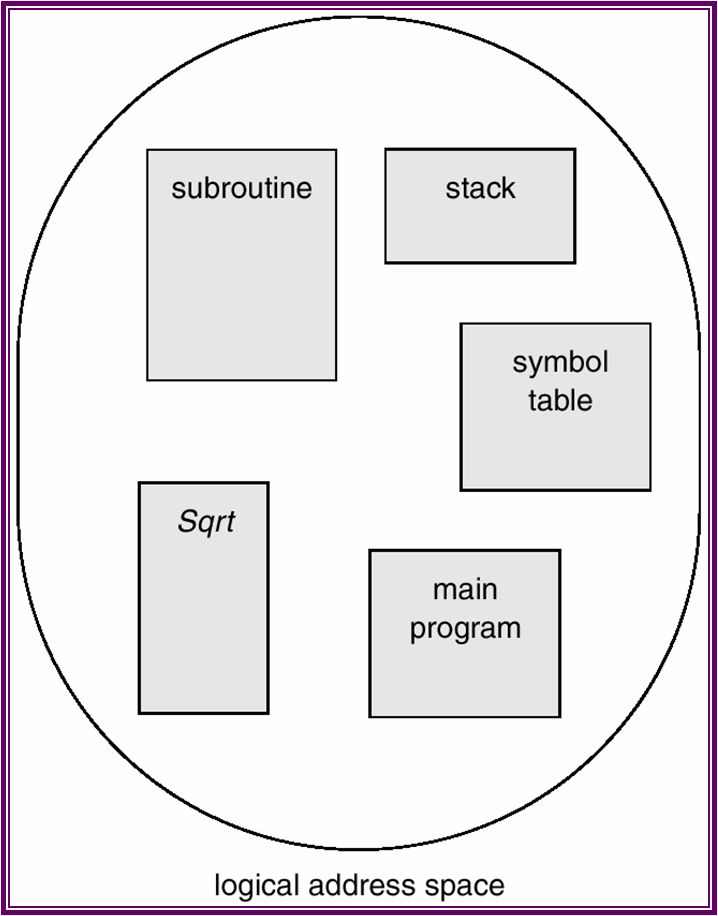
\includegraphics[scale=.5]{v6f9-17} \pause
  \end{minipage}%
  \begin{minipage}[c]{0.5\textwidth}
    \setlength{\unitlength}{.5cm}
    \centering
    \begin{picture}(5, 15)
      \put(1, 0){\framebox(5, 2){code}}
      \put(1, 2){\framebox(5, 2){data}}
      \put(1, 4){\framebox(5, 3){heap}}
      \put(1, 7){\framebox(5, 2){free}}
      \put(1, 9){\framebox(5, 2){stack}}
      \put(5, 6){\vector(0, 1){2}}
      \put(2, 10){\vector(0, -1){2}}
    \end{picture}
  \end{minipage}
  \end{frame}
  
  %% PAGE
  \begin{frame}
  \frametitle{User's view of memory(2/2)} \pause
  \begin{itemize}
  \item{与分页系统一样,这些段在物理内存中也不一定是连续的,如图所示:} \pause
  \end{itemize}
  \begin{center}
    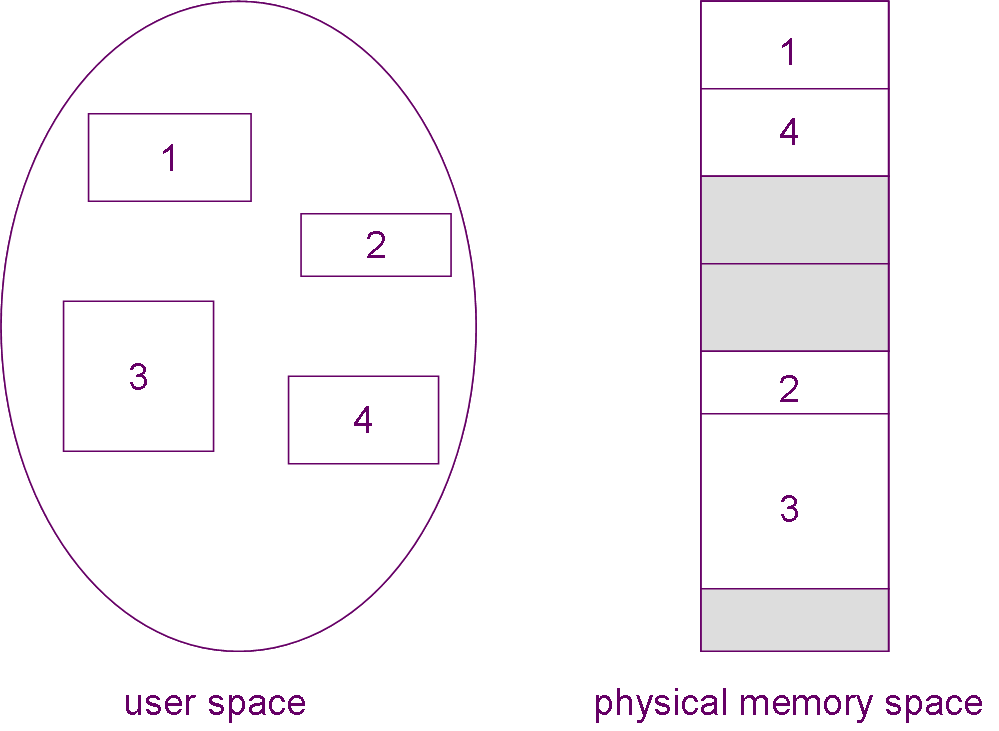
\includegraphics[scale=.5]{logicalviewofmemory}
  \end{center}
  \end{frame}
  
  %% PAGE
  \begin{frame}
  \frametitle{实现} \pause
  \begin{itemize}
  \item{Logical address consists of two parts: \\ $<$segment-number, offset$>$ } \pause
  \item{\textbf{Segment table} is used to map logical address to physical address. Each table entry has} \pause
    \begin{itemize}
    \item{\textbf{base} - contains the starting physical address where the segments reside in memory; } \pause
    \item{\textbf{limit} - specifies the length of the segment; } \pause
    \item{\textbf{protection bits (RWX)} of the segment. } \pause
    \end{itemize}
  \item{\textbf{Segment-table base register (STBR)} points to the segment table's location in the memory.} \pause
  \item{\textbf{Segment-table length register (STLR)} indicates number of segments used by a process.}
  \end{itemize}
  \end{frame}
  
  %% PAGE
  \begin{frame}
  \frametitle{地址转换} \pause
  \begin{center}
    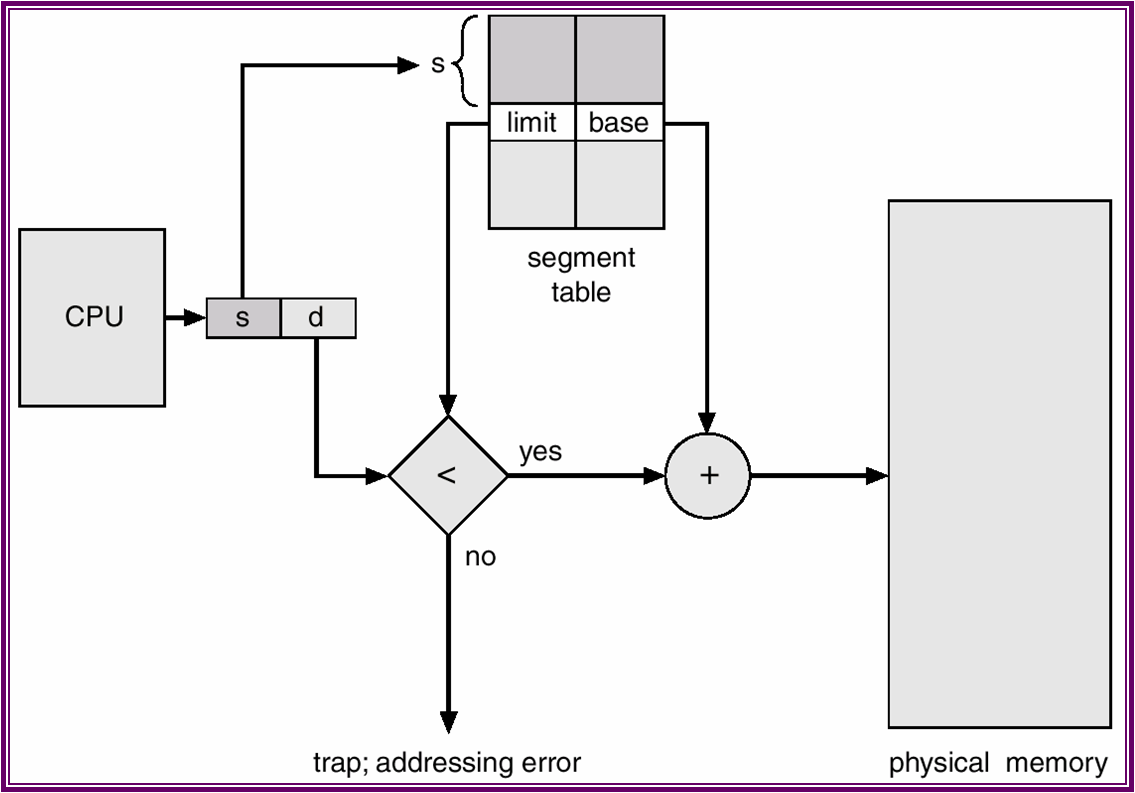
\includegraphics[scale=.5]{v6f9-18}
  \end{center}
  \end{frame}
  
  %% PAGE
  \begin{frame}
  \frametitle{例子} \pause
  \begin{center}
    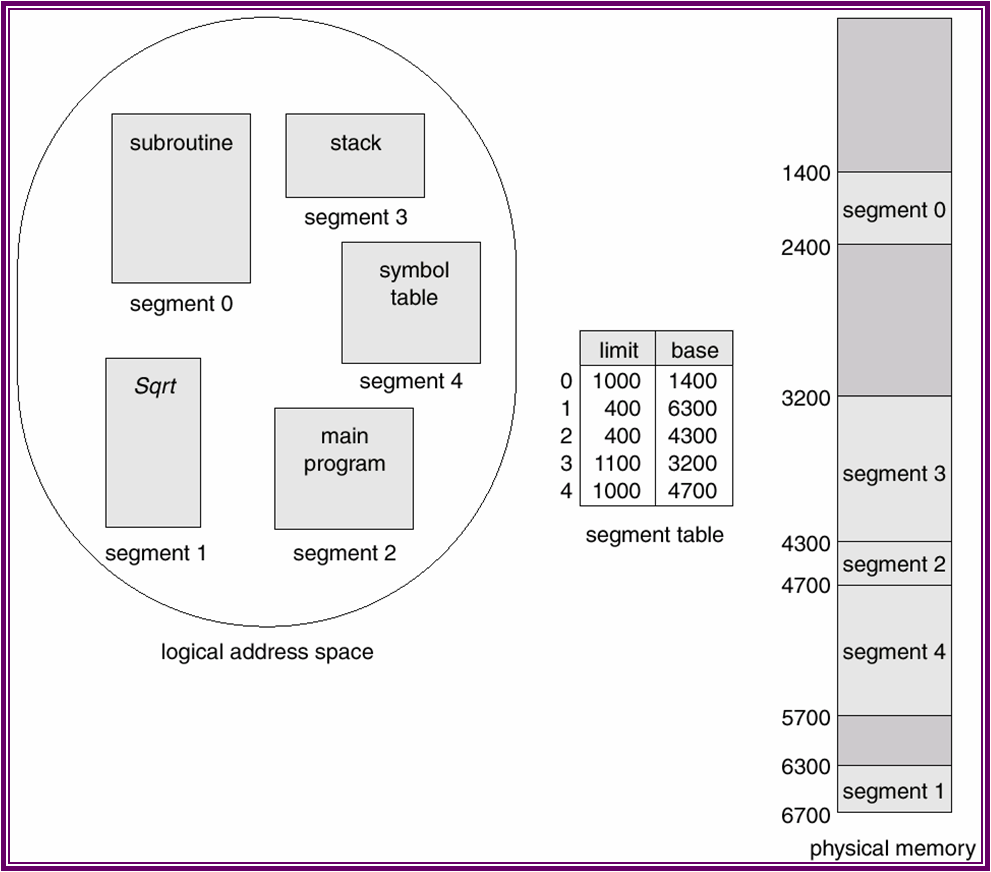
\includegraphics[scale=.5]{v6f9-19}
  \end{center}
  \end{frame}
  
  %% PAGE
  \begin{frame}
  \frametitle{内存保护与共享} \pause
  \begin{itemize}
  \item{当然,在分段系统中,内存的保护与共享以段为单位。如图所示:} \pause
  \end{itemize}
  \begin{center}
    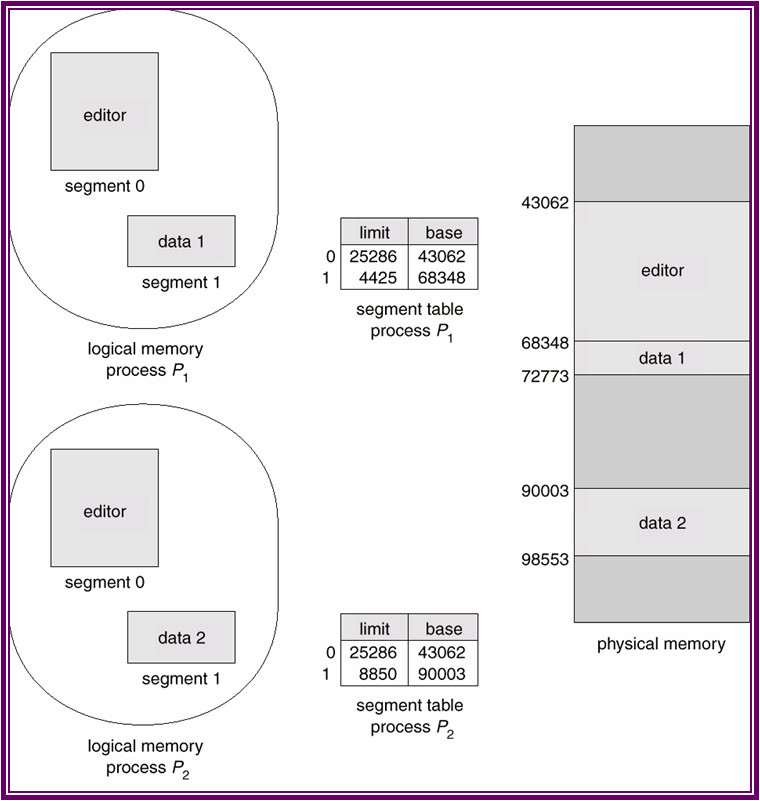
\includegraphics[scale=.5]{v6f9-20}
  \end{center}
  \end{frame}
  
  %% PAGE
  \begin{frame}
  \frametitle{结论} \pause
  \begin{itemize}
  \item{由于段的长度是根据需要变化的,因此分段会产生外部碎片。} \pause
    \begin{itemize}
    \item{这个问题的严重程度与操作系统的内存分配算法和进程各个段的平均大小有关。} \pause
    \end{itemize}
  \item{由于系统无法预测各个进程使用内存的状况,外部碎片很难控制。因此,单纯的分段系统目前很少使用。} \pause
  \item{各个硬件产商也不再支持单纯的分段系统。} \pause
    \begin{itemize}
    \item{INTEL 80386以前的CPU只支持分段,而80386以后(包括80386)的CPU则增加了分页支持。}
    \end{itemize}
  \end{itemize}
  \end{frame}
  
  %% PAGE
  \begin{frame}
  \frametitle{Questions}
  \begin{itemize}
  \item{Any questions?}
  \end{itemize}
  \begin{center}
    
\includegraphics[scale=.5]{question}
  \end{center}
  \end{frame}

\section{段页式内存管理}  
  
  %% PAGE
  \begin{frame}
  \frametitle{介绍} \pause
  \begin{itemize}
  \item{分页和分段系统有各自的优缺点,因此人们就考虑结合分页和分段,这就形成了段页式内存管理。} \pause
    \begin{itemize}
    \item{INTEL公司的IA-32(80386以后的CPU的统称,包含80386)是段页式内存管理的典范。} \pause
    \item{因此,下面我们以IA-32为例来讲解段页式内存管理。}
    \end{itemize}
  \end{itemize}
  \end{frame}
  
  %% PAGE
  \begin{frame}
  \frametitle{IA-32内存管理} \pause
  \begin{itemize}
  \item{在IA-32中,} \pause
    \begin{itemize}
    \item{分段是必须的} \pause
      \begin{itemize}
      \item{每个段最大可以为4GB。} \pause
%      \item{段被分成两种:全局段(global)和本地(私有)段(local)。} \pause
%        \begin{itemize}
%        \item{全局段最多可以有8K个,而每个进程可以有8K个私有段。} \pause
%        \end{itemize}
      \item{段表项被称为描述符(descriptor),相应地段表被称为描述符表(descriptor table);} \pause
      \item{逻辑地址$<$segment-number, offset$>$中的“segment-number”被称为段选择子(segment selector, 简称selector)。} \pause
      \end{itemize}
    \end{itemize}
  \item{而分页是可选的} \pause
    \begin{itemize}
    \item{页面和frame大小为4KB,采用二级页表。}
    \end{itemize}
  \end{itemize}
  \end{frame}
  
  %% PAGE
  \begin{frame}
  \frametitle{地址转换(1/3)} \pause
  \begin{itemize}
  \item{段页式内存管理的地址转换包括两个步骤:先分段,再分页。} \pause
    \begin{itemize}
    \item{下图给出了分段部分的地址转换。} \pause
    \end{itemize}
  \end{itemize}
  \begin{center}
    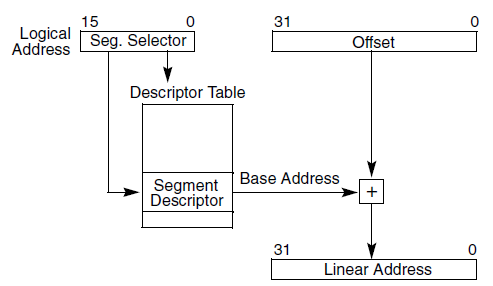
\includegraphics[scale=.5]{x86atl2l} \pause
  \end{center}
  \begin{itemize}
  \item{图中的“Linear Address”是逻辑地址经分段系统转换后的地址。} \pause
    \begin{itemize}
    \item{如果CPU关闭了分页功能,它就直接作为物理地址发到地址总线;} \pause
    \item{否则,它将继续被分页系统转换成物理地址。}
    \end{itemize}
  \end{itemize}
  \end{frame}
  
  %% PAGE
  \begin{frame}
  \frametitle{地址转换(2/3)} \pause
  \begin{itemize}
  \item{下图是前面见过的分页地址转换:} \pause
  \end{itemize}
  \begin{center}
    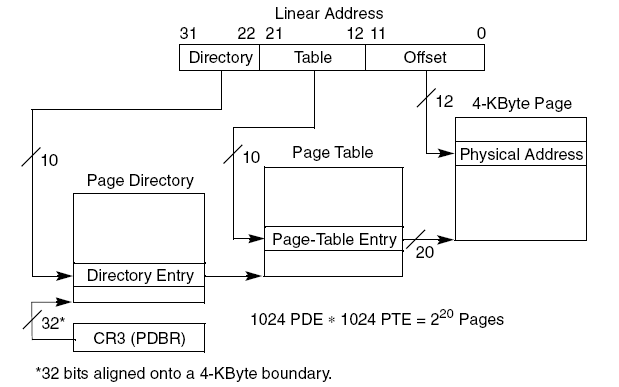
\includegraphics[scale=.5]{x86atl2p}
  \end{center}
  \end{frame}
  
  %% PAGE
  \begin{frame}
  \frametitle{地址转换(3/3)} \pause
  \begin{itemize}
  \item{Put them all together} \pause
  \end{itemize}
  \begin{center}
    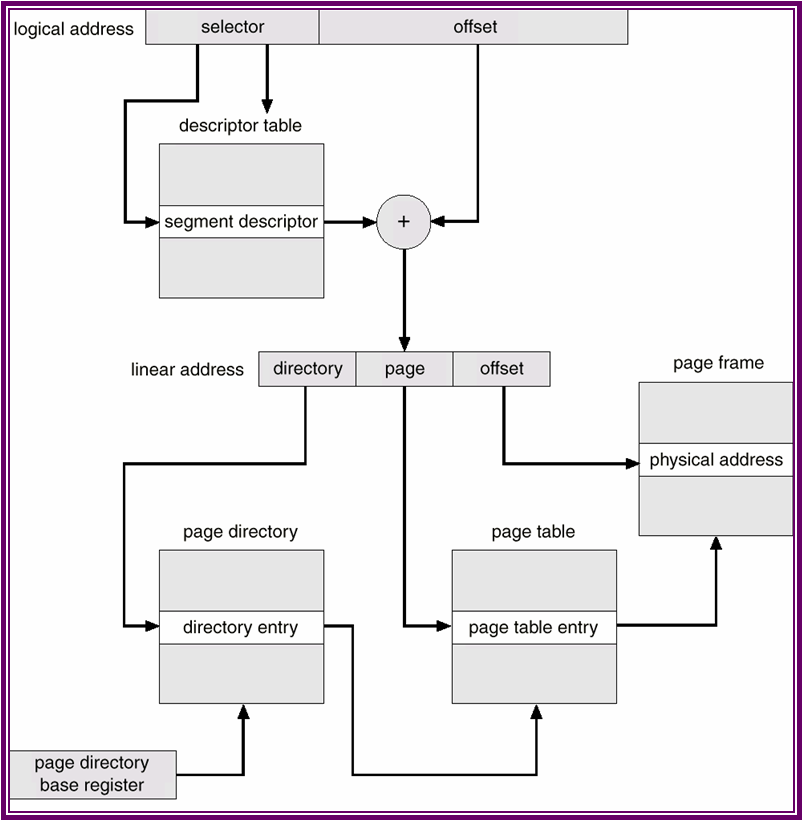
\includegraphics[scale=.5]{v6f9-21}
  \end{center}
  \end{frame}

\iffalse
  
  %% PAGE
  \begin{frame}
  \frametitle{段选择子(selector)} \pause
  \begin{itemize}
  \item{下图是段选择子的结构:} \pause
  \end{itemize}
  \begin{center}
    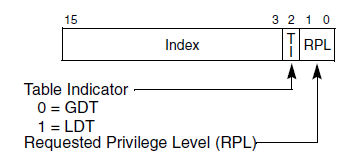
\includegraphics[scale=.5]{x86selector} \pause
  \end{center}
  \begin{itemize}
  \item{其中的TI字段确定了index所索引的段表是全局段表(GDT, Global Descriptor Table)或进程私有段表(LDT, Local Descriptor Table)。}
  \end{itemize}
  \end{frame}
  
\fi
  
  %% PAGE
  \begin{frame}
  \frametitle{段描述符(descriptor)} \pause
  \begin{center}
    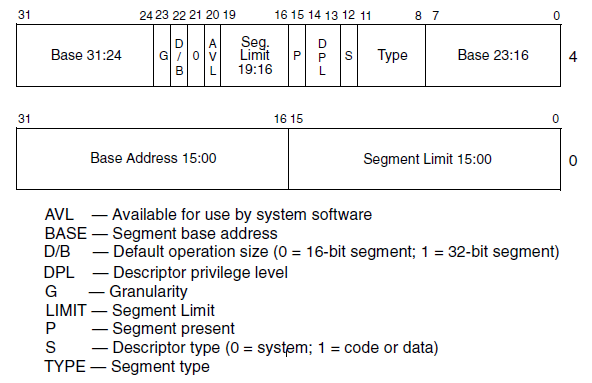
\includegraphics[scale=.5]{x86sd}
  \end{center}
  \end{frame}
  
  %% PAGE
  \begin{frame}
  \frametitle{Questions}
  \begin{itemize}
  \item{Any questions?}
  \end{itemize}
  \begin{center}
    
\includegraphics[scale=.5]{question}
  \end{center}
  \end{frame}
    
\end{CJK*}
\end{document}
